\documentclass[12pt, oneside]{scrreprt}
\usepackage{geometry}
\usepackage{hyperref}
\geometry{letterpaper}
\usepackage{graphicx}

\subject{Web Data - CS 483}
\title{Whoosh Indexing Report}
\subtitle{Super Clever Team Name}
\author{Aaron Goin\\Giselle Gomez\\Richie Zhang}
\date{Mar 10th 2017}	
\begin{document}
\maketitle

\pagebreak

\section*{Introduction}
For Assignment 3 our team was to create a search index using Whoosh! over our previously collected datasets and to allow searching the index from the command-line. Our dataset was obtained from Wikipedia and comprised of all stubs contained within the Confections, Desserts, and Fruit categories. We wrote one script to scrape and parse the xml data into a SQL database. We then wrote another script to index the data with Whoosh! without stemming the attributes. To make up for the lack of stemming, we use query.Variations in our Query Parser which calculates word variations for every term the user enters and broadens our search net.

\section*{Database}
\subsection*{Schema}
Our SQL database consisted of three tables with identical schemas: \\

\begin{center}
 \begin{tabular}{|l c ||}
    \hline
    Category \\
    \hline
    Name: STRING \\
    Image: STRING \\
    Description: STRING \\
    Source: STRING \\
    \hline
  \end{tabular} \\
\end{center}

Our Whoosh! indexed database combined the three tables into a single index with a simple schema: \\

\begin{center}
  \begin{tabular}{|l c ||}
    \hline
    Index \\ \hline
    Name: TEXT \\
    Category: TEXT \\
    Image: TEXT \\
    Description: TEXT \\
    Source: TEXT \\
    \hline
  \end{tabular}
\end{center} 

Both Image and Source are string URLs

\subsection*{Size}
Our database contains 1077 tuples in total, with 403 Desserts, 372 Sweets, and 302 Fruits.
\begin{figure}
    \centering
    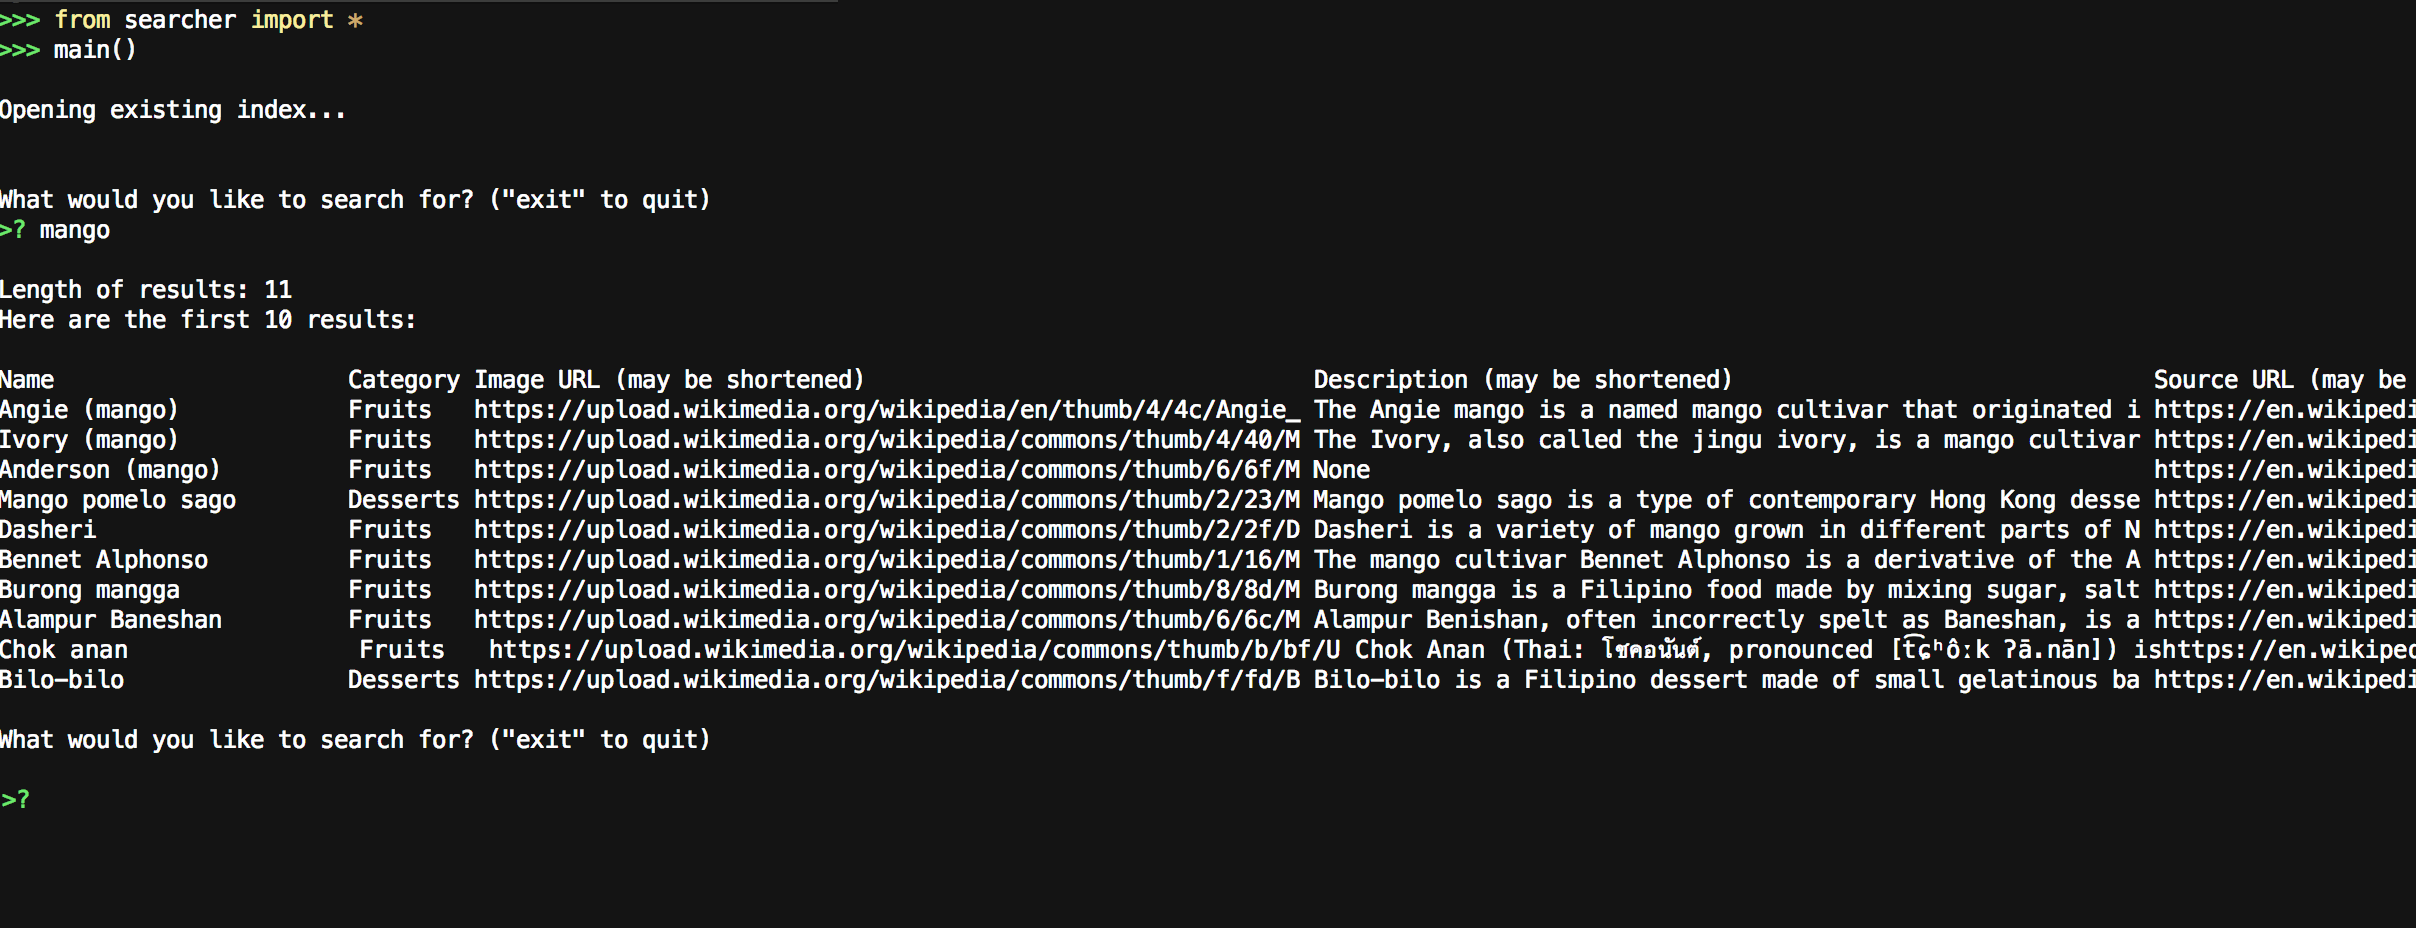
\includegraphics[width=\linewidth]{screenshotTwo.png}
    \caption{Screenshot of a an example of a search. This searches the index for mango.}
    \label{fig:my_label}
\end{figure}
\begin{figure}
    \centering
    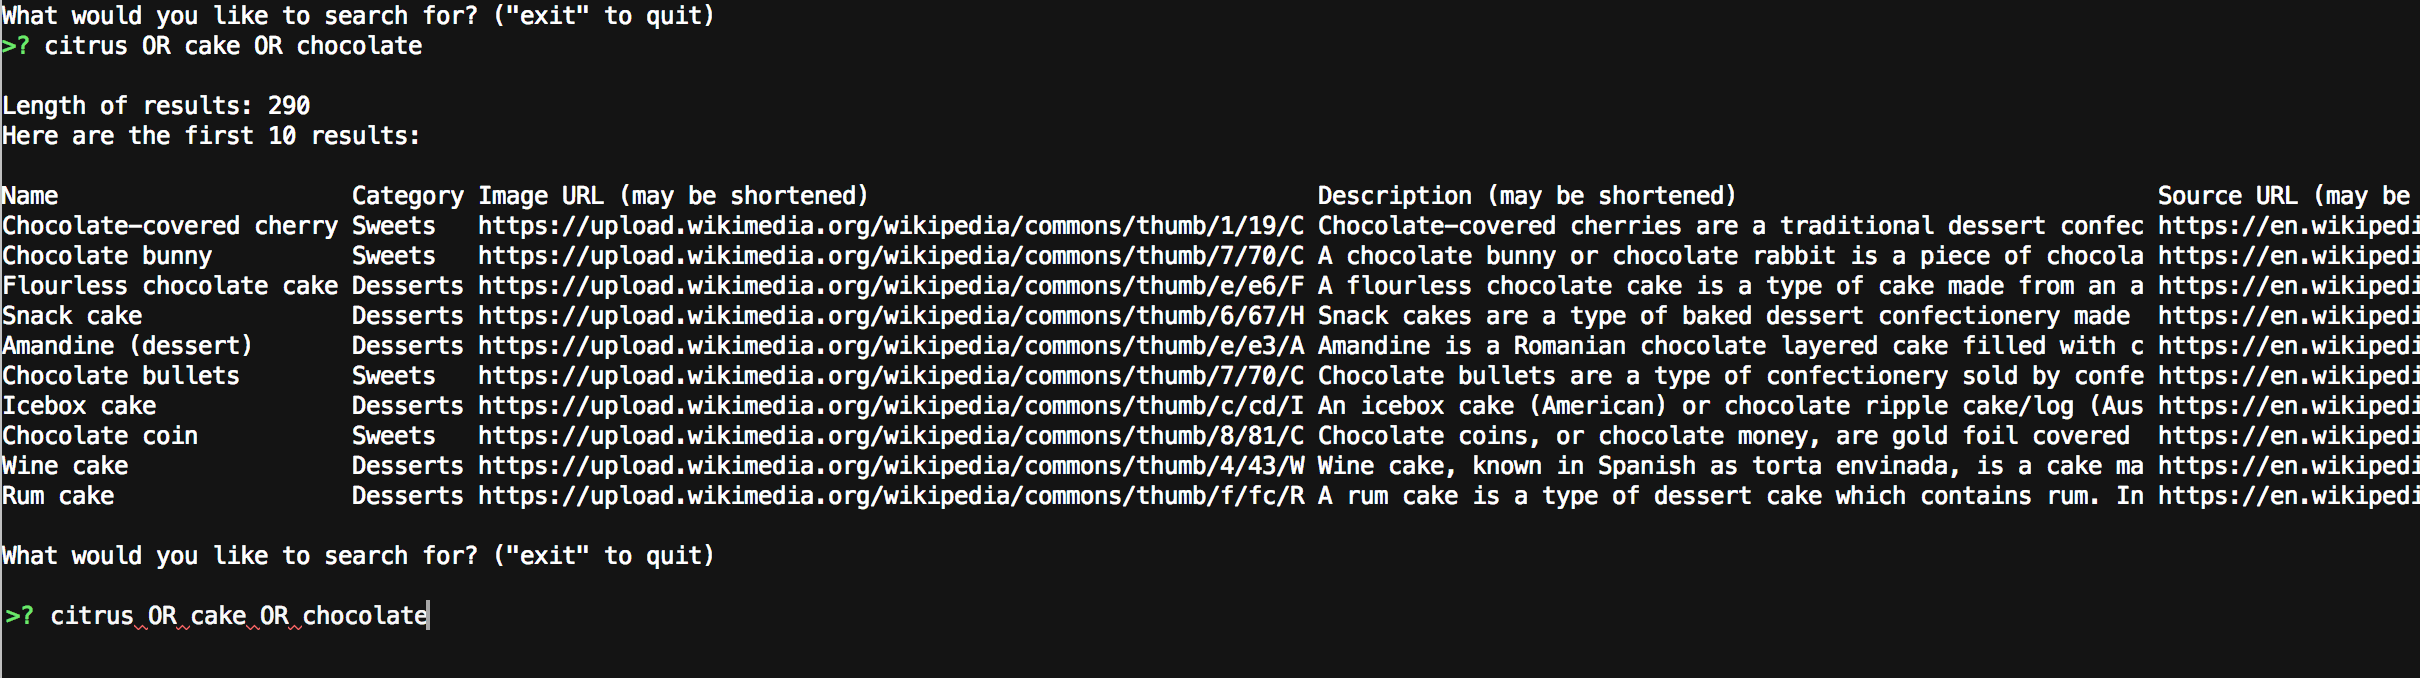
\includegraphics[width=\linewidth]{screenshotOne.png}
    \caption{Screenshot of a an example of a search. This searches the index for citrus OR cake OR chocolate.}
    \label{fig:my_label}
\end{figure}
\end{document}